%%%%%%%%%%%%%%%%%%%%%%%%%%%%%%%%%%%%%%%%%
% Jacobs Landscape Poster
% LaTeX Template
% Version 1.1 (14/06/14)
%
% Created by:
% Computational Physics and Biophysics Group, Jacobs University
% https://teamwork.jacobs-university.de:8443/confluence/display/CoPandBiG/LaTeX+Poster
% 
% Further modified by:
% Nathaniel Johnston (nathaniel@njohnston.ca)
%
% This template has been downloaded from:
% http://www.LaTeXTemplates.com
%
% License:
% CC BY-NC-SA 3.0 (http://creativecommons.org/licenses/by-nc-sa/3.0/)
%
%%%%%%%%%%%%%%%%%%%%%%%%%%%%%%%%%%%%%%%%%

%----------------------------------------------------------------------------------------
%	PACKAGES AND OTHER DOCUMENT CONFIGURATIONS
%----------------------------------------------------------------------------------------

\documentclass[final]{beamer}

\usepackage[scale=1.24]{beamerposter} % Use the beamerposter package for laying out the poster

%
%\usepackage[english]{babel}
%\usepackage[rflt]{floatflt}
%\usepackage{graphicx}
%\usepackage{url}
%\usepackage{multirow}
%\usepackage[rflt]{floatflt}
%\usepackage{graphicx}
%\usepackage{multirow}
\usepackage{supertabular}
%\usepackage{spverbatim}
%\usepackage{paralist}
%\usepackage{multicol}
%\usepackage{csquotes}
%\usepackage{flushend}
%\usepackage{cite}
%\usepackage{amsmath}
%\usepackage{amsfonts}
%\usepackage{amssymb}
\usepackage{pifont}
%\usepackage{booktabs}
%\usepackage{caption}
\usepackage{array}


%---------------------------------------------------------------------------------------
% Customised RHUL stuff
%---------------------------------------------------------------------------------------

% Some RHUL colours
\xdefinecolor{rhulgreen}{cmyk}{0.94,0,1,0}
\xdefinecolor{rhullime}{cmyk}{0.20,0,1,0.1}
\xdefinecolor{rhulyellow}{cmyk}{0,0.35,1,0}
\xdefinecolor{rhulred}{cmyk}{0,0.96,0.90,0}
\xdefinecolor{rhulpink}{cmyk}{0.12,1,0,0}
\xdefinecolor{rhulteal}{cmyk}{0.84,0,0.38,0}
\xdefinecolor{rhulsky}{cmyk}{0.86,0.08,0,0}
\xdefinecolor{rhulblue}{cmyk}{0.9,0.48,0,0}
\xdefinecolor{rhulpurple}{cmyk}{0.51,0.79,0,0}
\xdefinecolor{rhulorange}{cmyk}{0,0.7,1,0}%primary colour
\xdefinecolor{rhulgrey}{cmyk}{0.65,0.43,0.26,0.78}%primary colour


\usetheme{confposter} % Use the confposter theme supplied with this template

\setbeamercolor{block title}{fg=rhulorange,bg=white} % Colors of the block titles
\setbeamercolor{block body}{fg=rhulgrey,bg=white} % Colors of the body of blocks
\setbeamercolor{block alerted title}{fg=white,bg=rhulorange} % Colors of the highlighted block titles
\setbeamercolor{block alerted body}{fg=rhulgrey,bg=rhulorange!20} % Colors of the body of highlighted blocks
% Many more colors are available for use in beamerthemeconfposter.sty

% Many more colors are available for use in beamerthemeconfposter.sty

%-----------------------------------------------------------
% Define the column widths and overall poster size
% To set effective sepwid, onecolwid and twocolwid values, first choose how many columns you want and how much separation you want between columns
% In this template, the separation width chosen is 0.024 of the paper width and a 4-column layout
% onecolwid should therefore be (1-(# of columns+1)*sepwid)/# of columns e.g. (1-(4+1)*0.024)/4 = 0.22
% Set twocolwid to be (2*onecolwid)+sepwid = 0.464
% Set threecolwid to be (3*onecolwid)+2*sepwid = 0.708

\newlength{\sepwid}
\newlength{\onecolwid}
\newlength{\twocolwid}
\newlength{\threecolwid}
\setlength{\paperwidth}{48in} % A0 width: 46.8in
\setlength{\paperheight}{36in} % A0 height: 33.1in
\setlength{\sepwid}{0.024\paperwidth} % Separation width (white space) between columns
\setlength{\onecolwid}{0.22\paperwidth} % Width of one column
\setlength{\twocolwid}{0.464\paperwidth} % Width of two columns
\setlength{\threecolwid}{0.708\paperwidth} % Width of three columns
\setlength{\topmargin}{-0.5in} % Reduce the top margin size
%-----------------------------------------------------------

\usepackage{graphicx}  % Required for including images

\usepackage{booktabs} % Top and bottom rules for tables

%----------------------------------------------------------------------------------------
%	TITLE SECTION 
%----------------------------------------------------------------------------------------

\title{Towards Auditing of Control-Flow Integrity} % Poster title

\author[Your Name]{Luke Atherton { - Supervised by: Konstantinos Markantonakis}}

\institute{Information Security Group, Smart Card and IoT Security Center\\Royal Holloway, University of London} % Institution(s)

%----------------------------------------------------------------------------------------

\begin{document}

\addtobeamertemplate{block end}{}{\vspace*{1ex}} % White space under blocks
\addtobeamertemplate{block alerted end}{}{\vspace*{1ex}} % White space under highlighted (alert) blocks

\setlength{\belowcaptionskip}{2ex} % White space under figures
\setlength\belowdisplayshortskip{2ex} % White space under equations

\begin{frame}[t] % The whole poster is enclosed in one beamer frame

\begin{columns}[t] % The whole poster consists of three major columns, the second of which is split into two columns twice - the [t] option aligns each column's content to the top

\begin{column}{\sepwid}\end{column} % Empty spacer column

\begin{column}{\onecolwid} % The first column

%----------------------------------------------------------------------------------------
%	OBJECTIVES
%----------------------------------------------------------------------------------------

\begin{alertblock}{Objectives}

\begin{itemize}
\item Investigate existing method providing control-flow integrity;
\item Propose a solution for enabling the audit of control-flow integrity.
\end{itemize}

\end{alertblock}

%----------------------------------------------------------------------------------------
%	INTRODUCTION
%----------------------------------------------------------------------------------------

\begin{block}{Introduction}

\begin{itemize}
	\item Control-flow integrity is a useful measure of secure software execution; \vspace*{0.4cm}
	\item When using control-flow integrity as a policy is states that the execution flow of an application must follow the control-flow graph generated from the application; \vspace*{0.4cm}
	\item The problem of enforcing control-flow integrity can be approached from a three different directions: prevention, detection and attestation; \vspace*{0.4cm}
	\item In this paper, we intend to add a fourth method of enforcing control-flow integrity - audit. We will propose a solution which enables the tracking and storing of control-flow data in audit-friendly reports.
\end{itemize}

\end{block}

%----------------------------------------------------------------------------------------
%	PROTOCOL INITIALIZATION
%----------------------------------------------------------------------------------------

\begin{block}{Control-Flow Graphs}

Control-flow graphs (CFG) are a method used to formally describe the legitimate paths an application can take during execution. A simple of measure of control-flow integrity is to verify whether instructions are processed in an order which abides by the application's CFG.

CFGs consist of vertices - basic blocks, and edges - transition. Basic blocks represent a sequence of instructions which will always run from beginning to end. Transitions are made, for example, when a $jump$ occurs.

Transitions can take several forms:

\end{block}

\end{column} % End of the first column

%----------------------------------------------------------------------------------------
%	STOCK IMAGE
%----------------------------------------------------------------------------------------

\begin{column}{\sepwid}\end{column} % Empty spacer column

\begin{column}{\twocolwid} % Begin a column which is two columns wide (column 2)

%----------------------------------------------------------------------------------------
%	KEY AGREEMENT
%----------------------------------------------------------------------------------------

\begin{columns}[t,totalwidth=\twocolwid] % Split up the two columns wide column

\begin{column}{\onecolwid}\vspace{-.6in} % The first column within column 2 (column 2.1)

\begin{figure}
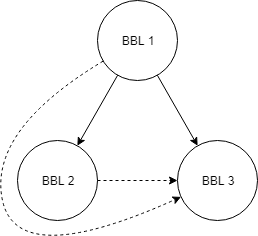
\includegraphics[width=\linewidth]{images/CFGIllegal.png}
\caption{Illegal control-flow}
\vspace{-1cm}
\end{figure}

\begin{block}{Control-Flow Integrity}

Control-flow integrity can be proved using several methods:


\textbf{Prevention} Theoretically CFI could not compromised. E.g. Read xor Write or deterministically encrypted instructions (ref).

\textbf{Detection} CFI compromise is detected during executions. E.g. stack canaries or shadow stacks (ref).

\textbf{Attestation} Variation of solutions have been examined, where control-flow is tracked at real time and used in an attestation protocol.
\end{block}

\begin{figure}
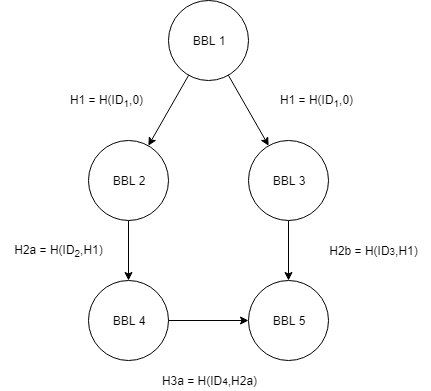
\includegraphics[width=\linewidth]{images/CFGhash.png}
\caption{CFG hash}
\vspace{-1cm}
\end{figure}

\end{column} % End of column 2.1

%----------------------------------------------------------------------------------------
%	EVALUATION
%----------------------------------------------------------------------------------------

\begin{column}{\onecolwid}\vspace{-.6in} % The second column within column 2 (column 2.2)

\begin{figure}
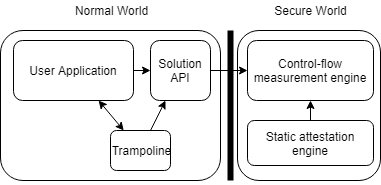
\includegraphics[width=\linewidth]{images/GraphicalRepresentation.png}
\caption{ARM TrustZone Implementation}
\vspace{-1cm}
\end{figure}

\begin{block}{Control-flow Monitoring}
We propose to insert x
\end{block}

\begin{figure}
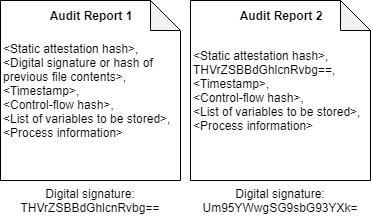
\includegraphics[width=\linewidth]{images/Files.png}
\caption{Audit files}
\vspace{-1cm}
\end{figure}

\begin{block}{Audit Files}
As well as containing the control-flow hash, the audit files will contain:
\begin{itemize}
	\item Initial attestation report; \vspace*{0.3cm}
	\item Digital signature of previous report; \vspace*{0.3cm}
	\item Operating environment information such as important variables and currently running processes.
\end{itemize}

\end{block}

\end{column} % End of column 2.2

\end{columns} % End of the split of column 2 - any content after this will now take up 2 columns width

\end{column} % End of the second column

%----------------------------------------------------------------------------------------
%	BENEFITS
%----------------------------------------------------------------------------------------

\begin{column}{\sepwid}\end{column} % Empty spacer column

\begin{column}{\onecolwid} % The third column

\begin{alertblock}{Benefits}

The proposed solutions enables the a new method of handling control-flow within embedded systems:
\begin{itemize}
\item Historic evidence of control-flow;
\item Binding of variables to control-flow snapshot;
\end{itemize}

\end{alertblock}

%----------------------------------------------------------------------------------------
%	CONCLUSION
%----------------------------------------------------------------------------------------
\vspace*{1cm}
\begin{block}{Conclusion}

Further work also

\end{block}

%----------------------------------------------------------------------------------------
%	REFERENCES
%----------------------------------------------------------------------------------------
\vspace*{1cm}
\begin{block}{References}

\nocite{*} % Insert publications even if they are not cited in the poster
\small{\bibliographystyle{unsrt}
\bibliography{bib}}

\end{block}

%----------------------------------------------------------------------------------------
%	CONTACT INFORMATION
%----------------------------------------------------------------------------------------

\setbeamercolor{block alerted title}{fg=white,bg=rhulorange} % Change the alert block title colors
\setbeamercolor{block alerted body}{fg=black,bg=white} % Change the alert block body colors

\begin{alertblock}{Contact Information}

\begin{itemize}
\item Web: \href{https://scc.rhul.ac.uk/}{https://scc.rhul.ac.uk/}
\item Email: \href{luke.atherton.2018@live.rhul.ac.uk}{luke.atherton.2018@live.rhul.ac.uk}
\item Twitter: @LucialHz
\end{itemize}

\end{alertblock}

%----------------------------------------------------------------------------------------

\end{column} % End of the third column

\end{columns} % End of all the columns in the poster

\end{frame} % End of the enclosing frame

\end{document}
